\section{Protecting against Malicious Retailers}
\label{sec:unlinkable-design-2}

The Basic Unlinkable CC Protocol is vulnerable to attacks by malicious retailers, as described in Section \ref{sec:secure-goals}.
In this section we describe the Secure Unlinkable CC Protocol to defend against these attacks, while continuing to support unlinkable transactions.

This new protocol is very similar to the Basic Unlinkable CC Protocol described in Section \ref{sec:unlinkable-design-1}.
In the Basic Unlinkable CC Protocol, a 93-bit token was used to identify a virtual credit card to the Wallet Server.
In the Secure Unlinkable CC Protocol, this token consists of only 80 bits, leaving 13 bits to bind a price to the token.
In binding a set price to a given token, we provide the same defense against malicious retailer attacks as the Secure CC Protocol described in Chapter \ref{cha:secure}.

When the Wallet Server receives a Registration message, it stores the card information and associates a card identifier \emph{Ident} with this record.
It also generates a secret key \emph{secret} associated with this card.
In the Secure Unlinkable CC Protocol, the Wallet Server responds to the Registration message with this identifier \emph{Ident} and the key \emph{SK}.
The Wallet Application stores these values securely, associating them with the credit card being registered.
The protocol, illustrated in Figure \ref{fig:unlinkable-2}, operates as follows:

\begin{figure}[h!]
  \caption{Secure Unlinkable CC Protocol}
  \centering
    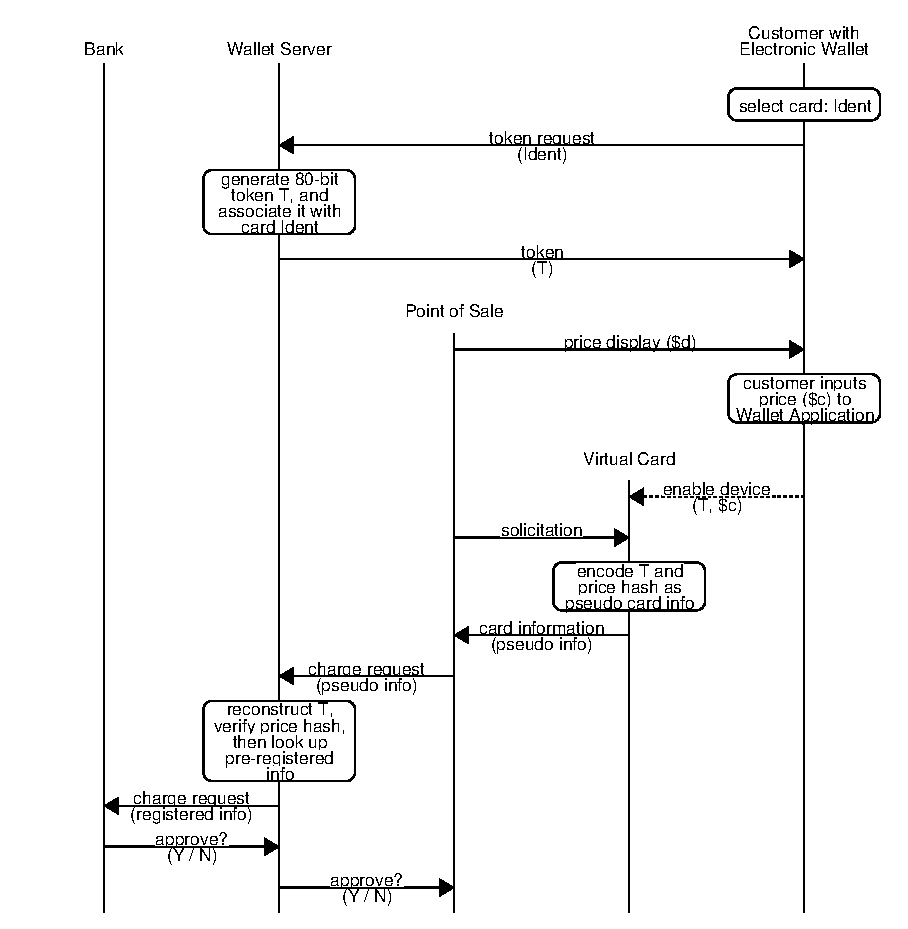
\includegraphics{img/unlinkable-2.eps}
  \label{fig:unlinkable-2}
\end{figure}

\begin{enumerate}
\item When the customer wishes to use a credit card, the customer selects a credit card in the Wallet Application.

\item The Wallet Application sends a Token Request message to the Wallet Server.
    This message consists of the card identifier \emph{Ident} associated with the selected card, and is sent securely over the Internet.
    Note that this message needs to be authenticated, to prevent a customer from requesting a token to a different customer's card.

\item The Wallet Server then generates a random 80-bit token \emph{T}, and associates it with the card identified by \emph{Ident}.
    The Wallet Server responds to the Wallet Application with a Token message containing \emph{T}.

\item The point of sale displays the price to charge (\$d) on its screen.

\item The customer enters the price to be charged (\$c) into the Wallet Application.

\item The Wallet Application now enables the virtual credit card, initializing it with token \emph{T} and price \$c.
    The virtual credit card begins listening for Solicitation messages.

\item The point of sale sends a Solicitation message to the virtual credit card over the NFC channel.

\item The virtual credit card calculates the hash of token \emph{T} combined with price \$c, keyed with key \emph{SK}, and selects the first 13 bits of this hash.
    It then combines the 80-bit token \emph{T} with this 13-bit hash to acquire a 93-bit value.
    Finally, it converts this 93-bit value into a 28-digit number \emph{k}, and responds with a pseudo Card Information message as before.

\item The point of sale constructs an Charge Request message from the (pseudo) Card number, Expiration date, iCVV, and the price it wishes to charge.
    This message is sent to the bank named in the Card Information message.
    As a result, the Charge Request message is directed to the Wallet Server and \emph{not} an actual bank.
    Note that from the perspective of the point of sale, the Wallet Server appears to be a bank like any other.

\item The Wallet Server reconstructs \emph{k} from the Charge Request message, and computes the 80-bit token and 13-bit price hash that it represents.
    The Wallet Server then searches its database for the token, to identify the card used in this transaction.
    If the token is not found, the Wallet Server sends a ``declined'' Acceptance message to the point of sale, and aborts the protocol.
    Otherwise, the secret key \emph{SK} is retrieved from the Wallet Server's database, and the Wallet Server calculates its own version of the price hash
        using the price indicated by the point of sale in the Charge Request message.
    If the Wallet Server's price hash does not match the price hash in the Charge Request mesage,
        the Wallet Server sends a ``declined'' Acceptance message to the point of sale and aborts the protocol.
    Otherwise, the stored card information is retrieved from the Wallet Server's database.
    The Wallet Server invalidates the token, and sends a \emph{visual} Charge Request to the card's bank with the following fields:
    \begin{itemize}
    \item Cardholder name
    \item Card number
    \item Expiration date
    \item Billing address
    \end{itemize}
    Note that unlike the Card Information message sent by the Wallet Application, this data reflects the actual credit card information,
        acquired by the Wallet Server during the card registration.

\item The bank receives the \emph{visual} Charge Request from the Wallet Server, and processes this transaction as normal.
    The bank then responds to the Wallet Server with an Acceptance message indicating whether the charge has been accepted.

\item The Wallet Server forwards the bank's Acceptance message to the point of sale.
\end{enumerate}

In the Secure Unlinkable CC Protocol, the Card Information messages are bound to the price entered by the customer:
    a malicious retailer, lacking knowledge of \emph{SK}, cannot generate a replacement price hash should it charge a different price in the Charge Request message.
This protocol is also unlinkable: all 93 bits represented by the (pseudo) Card Information values are indistinguishable from random to the retailer.

However, like in the Basic Unlinkable CC Protocol, the Wallet Application needs to have a ready connection to the Internet.
Once a token has been used, a subsequent token must be acquired from the Wallet Server in order to make subsequent purchases.